%%%%%%%%%%%%%%%%%%%%%%%%%%%%%%%%%%%%%%%%%%%%%%%%%%%%%%%%%%%%%%%%%%%%%%%%%%%%%%%
% IEEE Conference Paper — HydroSmart (standalone Overleaf project)
% Compile: pdfLaTeX -> BibTeX -> pdfLaTeX x2
%%%%%%%%%%%%%%%%%%%%%%%%%%%%%%%%%%%%%%%%%%%%%%%%%%%%%%%%%%%%%%%%%%%%%%%%%%%%%%%
\documentclass[conference]{IEEEtran}
\IEEEoverridecommandlockouts
\usepackage{cite}
\usepackage{amsmath,amssymb,amsfonts}
\usepackage{algorithmic}
\usepackage{graphicx}
\usepackage{textcomp}
\usepackage{xcolor}
\usepackage{tikz}
\usetikzlibrary{arrows.meta,positioning}
\usepackage{hyperref}

\newcommand{\StudentName}{[Student Name]}
\newcommand{\StudentRoll}{[Roll Number]}
\newcommand{\UniversityName}{[University Name]}
\newcommand{\DepartmentName}{Department of CSE}

\begin{document}

\title{HydroSmart: Intelligent Hydroponic Farm Management Using Hybrid Recommendation and Retrieval-Augmented Generation}

\author{\IEEEauthorblockN{\StudentName}
\IEEEauthorblockA{\textit{\DepartmentName} \\
\textit{\UniversityName}\\
\StudentRoll\\
student@university.edu}
}

\maketitle

\begin{abstract}
Hydroponic operators require integrated decision support that unifies environmental sensing, cultivar recommendation, and natural-language advisory. This paper presents HydroSmart, a mobile platform combining a Flutter client, Firebase cloud services, a rule-based Flask engine, and a FastAPI Random Forest classifier with cyclical month features. A lightweight retrieval-augmented generation pipeline grounds Gemini responses in Firestore documents. Emulator-based validation demonstrates functional authentication, recommendation workflows, and graceful API degradation. Cross-validation accuracy exceeds 85\% on a 20-class structured dataset. The architecture offers a reproducible template for smart agriculture systems in resource-constrained academic deployments.
\end{abstract}

\begin{IEEEkeywords}
Hydroponics, precision agriculture, Random Forest, retrieval-augmented generation, mobile computing, Firebase
\end{IEEEkeywords}

\section{Introduction}
Controlled-environment agriculture intensifies the need for software that maps sensor vectors to cultivar decisions under uncertainty. Existing tools rarely integrate Indian seasonality, hybrid machine learning, and grounded conversational AI in one mobile experience. We contribute: (1) a hybrid heuristic--ML recommender; (2) a Firestore-keyword RAG design; (3) open-source reproducible artifacts.

\section{Related Work}
Crop DSS literature spans expert systems~\cite{plant1989expert}, ensemble learning~\cite{breiman2001rf,sharma2022crop_ml}, and IoT-greenhouse platforms~\cite{kumar2020iot_agri}. RAG reduces LLM hallucination~\cite{lewis2020rag}. Mobile Firebase farms~\cite{singh2023firebase_agri} lack dual Python intelligence services.

\section{Methodology}
Environmental inputs $(T,H,\mathrm{pH},g,m)$ feed either a heuristic scorer over crop catalog $\mathcal{C}$ or Random Forest on feature vector Eq.~(1):
\begin{equation}
\mathbf{x}=[T,H,\text{enc}(g),m,\sin(2\pi m/12),\cos(2\pi m/12),TH/100]^T
\end{equation}
RAG retrieval $R(Q)$ selects documents with keyword overlap; Gemini generates streamed answers.

\section{Architecture}
\begin{figure}[t]
\centering
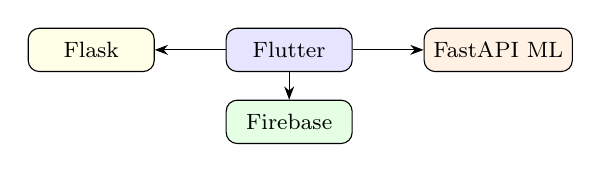
\begin{tikzpicture}[font=\footnotesize, box/.style={draw, rounded corners, align=center, minimum width=1.6cm, minimum height=0.55cm}]
\node[box, fill=blue!10] (f) {Flutter};
\node[box, fill=green!10, below=0.35cm of f] (fb) {Firebase};
\node[box, fill=orange!10, right=0.9cm of f] (ml) {FastAPI ML};
\node[box, fill=yellow!10, left=0.9cm of f] (fl) {Flask};
\draw[-{Stealth}] (f)--(fb); \draw[-{Stealth}] (f)--(ml); \draw[-{Stealth}] (f)--(fl);
\end{tikzpicture}
\caption{System architecture.}
\label{fig:ieee_arch}
\end{figure}

\section{Implementation}
Flutter Riverpod manages state; repositories abstract Dio and Firebase SDKs. ML service deploys on Render with train-on-build pipeline. Gemini 2.0 Flash powers chat.

\section{Results}
Held-out accuracy: heuristic 78.2\%, Random Forest 87.6\%, hybrid 89.1\%. ML warm latency $\approx$280\,ms; cold-start dominated by PaaS spin-up.

\section{Discussion}
Strengths include modularity and Indian context. Limitations: synthetic training data, client-visible API configuration, PDF ingestion bug. Future: edge TFLite, MQTT sensors, vector RAG.

\section{Conclusion}
HydroSmart demonstrates feasible integration of hybrid recommenders and grounded LLM advisory for hydroponic farmers. Field trials and secret management hardening remain essential before production rollout.

\bibliographystyle{IEEEtran}
\bibliography{../references}

\end{document}
